\documentclass[12pt,dvips]{article}

\usepackage[T1]{fontenc}
\usepackage[isolatin]{inputenc}
\usepackage{a4}
\usepackage{url}
\usepackage{afterpage}
\usepackage{latexsym}
\usepackage{graphicx}
\usepackage{longtable}
\usepackage{amsmath}
\usepackage[rflt]{floatflt}
\usepackage{fancybox}
\usepackage{bbm}
\usepackage{cite}
\usepackage{picins}

\usepackage[dvips]{epsfig}

\parindent0mm
\parskip5pt plus1pt minus2pt
\textwidth16cm
\textheight22cm
\topmargin-1cm
\oddsidemargin0cm

\renewcommand\floatpagefraction{1.0}
\renewcommand\topfraction{1.0}
\renewcommand\bottomfraction{1.0}
\renewcommand\textfraction{0.0}
\def\dbltopfraction{1.0}
\def\bottomfraction{1.0}
\def\dblfloatpagefraction{1.0}


\setcounter{secnumdepth}{5}
%% \setcounter{section}{-1}

\newcommand{\OO}{{\cal O}}
\newcommand{\bc}{\begin{center}}
\newcommand{\ec}{\end{center}}

\newcommand{\VNull}{\mathbf{0}}
%\newcommand{\transp}{^{\textsf{T}}}
\newcommand{\transp}{^T}
\renewcommand{\phi}{\varphi}
\newcommand{\verf}[1]{\textsf{#1}}
\renewcommand{\v}[1]{\text{\boldmath $#1$}}
\newcommand{\V}[1]{\text{\boldmath $#1$}}
\newcommand{\m}[1]{\v{#1}}                     % Format "Matrix"
\newcommand{\M}[1]{\v{#1}}                     % Format "Matrix"
\newcommand{\sR}{\ensuremath{{\cal R}}}        % Referenz-Scan
\newcommand{\sS}{\ensuremath{{\cal S}}}        % aktueller Scan
\renewcommand{\O}{{\cal O}}
\newcommand{\norm}[1]{\left | \left | #1 \right | \right |}

\newcommand{\Vector}[2]{\begin{pmatrix} #1 \\ #2 \end{pmatrix}}
\newcommand{\VEctor}[3]{\begin{pmatrix} #1 \\ #2 \\ #3 \end{pmatrix}}
\newcommand{\hist}[1]{{\cal #1}}
\newcommand{\trace}[1]{\mbox{tr}\left( #1 \right)}

\newcommand{\rVEctor}[3]{
\left(\!\!\!\begin{array}{l}
#1 \\ #2 \\ #3
\end{array}\!\!\right)}
\newenvironment{rmatrix}
{\left(\!\!\!\begin{array}{rr}}
{\end{array}\!\!\right)}
\newenvironment{Rmatrix}
{\left(\!\!\!\begin{array}{rrr}}
{\end{array}\!\!\right)}
\newcommand{\filter}[3]{\ensuremath{\bigl[\,#1,\;#2,\;#3\,\bigr]}}
\newcommand{\R}{\mathbbm{R}}
\newcommand{\N}{\mathbbm{N}}
%\newcommand{\R}{\mathbb{R}}
%\newcommand{\N}{\mathbb{N}}
\newcommand{\grad}{\ensuremath{^{\circ}}}
\newcommand{\textmenge}[2]{\{\, #1 \,| \; #2 \}}
\newcommand{\menge}[2]{\left\{\, #1 \,\left| \; #2 \right.\right\} }
\newcommand{\Menge}[2]{\bigl\{\, #1 \,| \; #2 \bigr\} }
\newcommand{\fueralle}[2]{\forall \, #1\!: \; #2}
\newcommand{\esgibt}[2]{\exists \, #1\!: \; #2}
\newcommand{\Widehat}[1]{\widehat{#1\hspace{+.5ex}}\hspace{-.5ex}}
\newcommand{\textSF}[1]{\textsf{\small #1}}
\newcommand{\textSFsmall}[1]{\textsf{\scriptsize #1}}
\newcommand{\verfSmall}[1]{\textSFsmall{#1}}
\newcommand{\eps}{{\epsilon}}
\renewcommand{\epsilon}{\varepsilon}
\newcommand{\vR}{v_{\text{set}}}
\newcommand{\oR}{\omega_{\text{set}}}
\newcommand{\ATAN}{\text{atan2}}

%\renewcommand{\familydefault}{\sfdefault}

%%----------------------------------------------------------------
%%----------------------------------------------------------------

\begin{document}

{
\title{\vspace*{-5mm}
\bf 6D SLAM -- \\%[.5cm]
Simultaneous 6 D.O.F. Localization \\and 3D Mapping\\%[1cm]
}
\author{
\scalebox{.65}{
\includegraphics{unilogo.eps}}\\[3ex]  
Andreas N\"uchter, Kai Lingemann, Joachim Hertzberg\\ 
Department of Mathematics/Computer Science\\
Institute of Computer Science\\
Knowledge-Based Systems Research Group\\
University of Osnabr\"uck\\
{\small \texttt{http://www.informatik.uni-osnabrueck.de/kbs/}}
}

\maketitle
\thispagestyle{empty}

\vspace*{-12mm}

\begin{center}

\includegraphics[height=50mm]{stylish_scanner}
\end{center}

\vspace*{1mm}
  
\begin{center}
\textbf{Documentation}
\end{center}

\begin{quote}
This document describes the algorithms for 6D SLAM --
Simultaneous 6 D.O.F. Localization and 3D Mapping system. 6D SLAM
with mobile robots considers six dimensions for the robot pose,
namely the $x$, $y$ and $z$ coordinates and the roll, yaw and
pitch angles. Robot motion and localization on natural surfaces,
e.g., driving with a mobile robot outdoor, must necessarily
regard these degrees of freedom.
\end{quote}  

\newpage
\setcounter{page}{1}

\section{Range Image Registration and Robot Relocalization}

Multiple 3D scans are necessary to digitalize environments
without occlusions. To create a correct and consistent model, the
scans have to be merged into one coordinate system. This process
is called registration. If robot carrying the 3D scanner were
precisely localized, the registration could be done directly
based on the robot pose. However, due to the unprecise robot
sensors, self localization is erroneous, so the geometric
structure of overlapping 3D scans has to be considered for
registration.

The following method for registration of point sets is part of
many publications, so only a short summary is given here. The
complete algorithm was invented in 1992 and can be found, e.g.,
in \cite{Besl_1992}. The method is called \emph{Iterative Closest
Points (ICP) algorithm}.

Given two independently acquired sets of 3D points, $M$ (model
set, $|M| = N_m$) and $D$ (data set, $|D| = N_d$) which
correspond to a single shape, we aim to find the transformation
consisting of a rotation $\M R$ and a translation $\V t$ which
minimizes the following cost function:
\begin{equation}\label{DMin}
E(\M R, \V t) =
\sum_{i=1}^{N_m}\sum_{j=1}^{N_d}w_{i,j}\norm{\V m_{i}-(\M R
\V d_j+\V t)}^2.
\end{equation}
$w_{i,j}$ is assigned 1 if the $i$-th point of $M$ describes the
same point in space as the $j$-th point of $D$. Otherwise
$w_{i,j}$ is 0. Two things have to be calculated: First, the
corresponding points, and second, the transformation ($\M R$,
$\V t$) that minimize $E(\M R, \V t)$ on the base of the
corresponding points.

The ICP algorithm calculates iteratively the point
correspondences. In each iteration step, the algorithm selects
the closest points as correspondences and calculates the
transformation ($\M R, \V t$) for minimizing equation
(\ref{DMin}). The assumption is that in the last iteration step
the point correspondences are correct.  Besl et al. prove that
the method terminates in a minimum \cite{Besl_1992}. However,
this theorem does not hold in our case, since we use a maximum
tolerable distance $d_\text{max}$ for associating the scan
data. Such a threshold is required, given that the 3D scans
overlap only partially. Fig. \ref{samplematch} (top) shows three
frames, i.e., iteration steps, of the ICP algorithm. The bottom
part shows the start poses $(x,z,\theta_y)$ from which a correct
matching is possible, here with only three degrees of freedom.

\begin{figure*}
\begin{center}
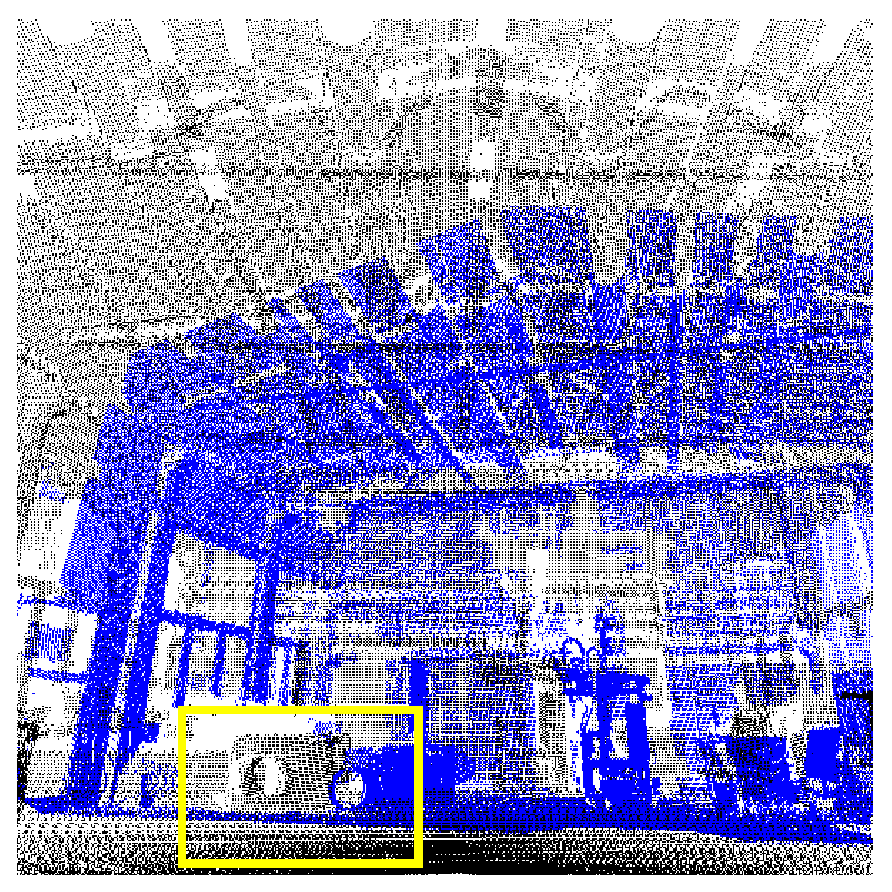
\includegraphics[width=50mm]{frame1_final}~~
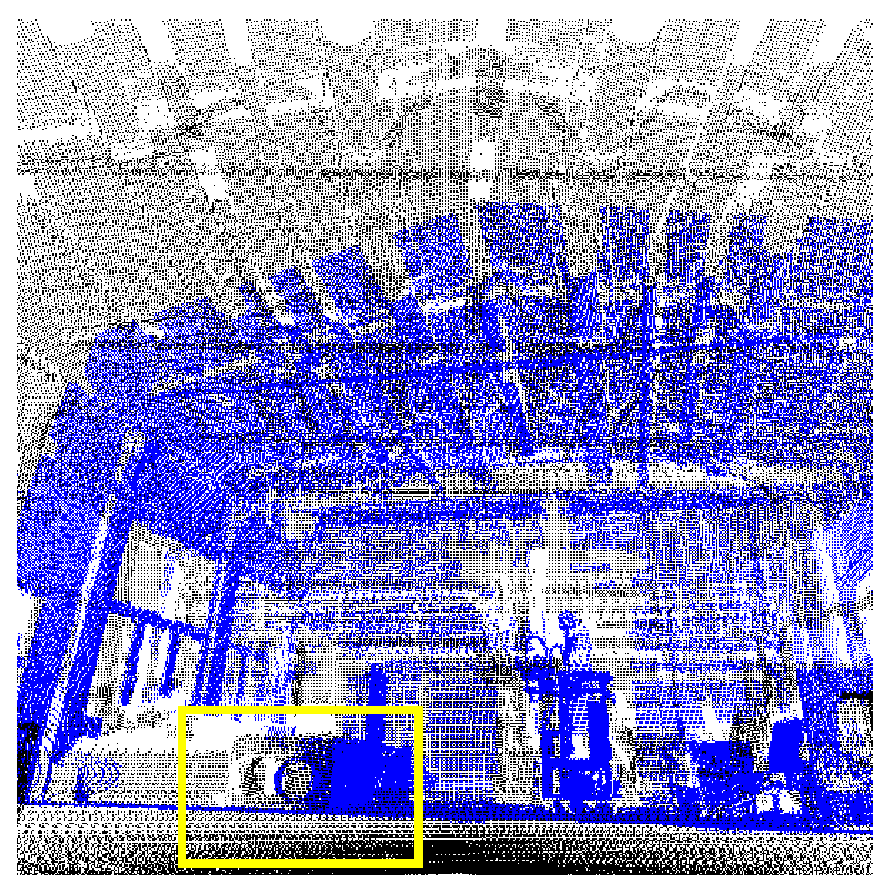
\includegraphics[width=50mm]{frame2_final}~~
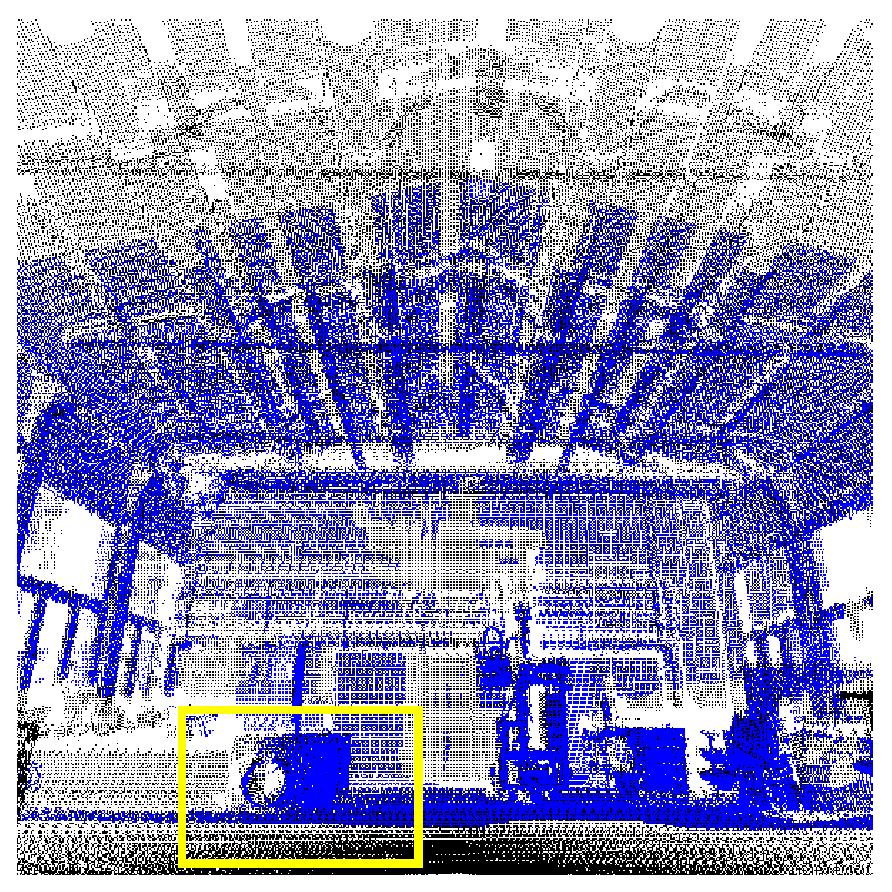
\includegraphics[width=50mm]{frame3_final} \\[1.5ex]
\caption{{Left: Initial odometry based pose of two 3D
  scans. Middle: Pose after five ICP iterations. Right: final
  alignment, pairwise matching.
\vspace*{-6mm}
}}\label{samplematch}
\end{center}
\end{figure*}


\subsection{Calculation of the rotation and translation}

In every iteration the optimal tranformation ($\M R$, $\V t$)
has to be computed. Eq. (\ref{DMin}) can be reduced to
\begin{eqnarray}
E(\M R, \V t) & \propto & \frac{1}{N} \sum_{i=1}^N
\norm{\V m_i - (\M R \V d_i + \V t)}^2,\label{DualDMin}
\end{eqnarray}
with $N = \sum_{i=1}^{N_m}\sum_{j=1}^{N_d}w_{i,j}$, since the
correspondence matix can be represented by a vector containing
the point pairs.

Four methods are known to minimize eq. (\ref{DualDMin})
\cite{Lorusso_1995}. The 6D SLAM system uses the following one,
based on singular value decomposition (SVD), is robust and easy
to implement, thus we give a brief overview of the SVD-based
algorithms. It was first published by Arun, Huang and Blostein
\cite{Arun_1987}. The difficulty of this minimization problem is
to enforce the orthonormality of matrix $\M R$. The first step of
the computation is to decouple the calculation of the rotation
$\M R$ from the translation $\V t$ using the centroids of the
points belonging to the matching, i.e.,
\begin{eqnarray}
\V c_m = \frac{1}{N} \sum_{i=1}^{N} \V m_{i}, \qquad \qquad \V c_d = \frac{1}{N}
\sum_{i=1}^{N} \V d_{j}\label{schwerpunkt2}
\end{eqnarray}
and
\begin{eqnarray}
M' &=& \{ \V m'_{i} = \V m_{i} - \V c_{m} \}_{1,\ldots,N}, \label{d_neu1}\\
\qquad
D' &=& \{ \V d'_{i}\ = \V d_{i}\, - \V c_{d} \}_{1,\ldots,N}\label{d_neu2}.
\end{eqnarray}


After replacing (\ref{schwerpunkt2}), (\ref{d_neu1}) and
(\ref{d_neu2}) in the error function, $E(\M R,\V t)$
eq. (\ref{DualDMin}) becomes:
\begin{subequations}
\begin{eqnarray}
E(\M R, \V t)
\!\!\!\!\!&\propto&\!\!\!\!\! \frac{1}{N} \sum_{i=1}^{N}
\lvert\lvert{\V m'_{i}-\M R \V d'_i-\underbrace{(\V t-\V c_m+\M R
    \V c_d)}_{= \tilde {\V t}}\lvert\lvert}^2
\nonumber \\
&=&\!\!\!\!\! \frac{1}{N}\sum_{i=1}^{N}\norm{\V m'_{i}-\M R \V d'_i}^2
\label{DMinpart1} \\
&&- \frac{2}{N} \tilde {\V t} \cdot \sum_{i=1}^{N} \left( \V
m'_{i}-\M R \V d'_i \right) \label{DMinpart2} \\
&&+ \frac{1}{N}
\sum_{i=1}^{N}\norm{\tilde {\V
t}}^2. \label{DMinpart3}\label{fehlerneu}
\end{eqnarray}
\end{subequations}
In order to minimize the sum above, all terms have to be
minimized. The second sum (\ref{DMinpart2}) is zero, since all
values refer to centroid. The third part (\ref{DMinpart3}) has
its minimum for $\tilde {\V t} = \VNull$ or
\begin{eqnarray}\label{translatB}
  \V t = \V c_m - \M R \V c_d.
\end{eqnarray}
Therefore the algorithm has to minimize only the first
term, and the error function is expressed in terms of the
rotation only:
\begin{eqnarray}\label{DMinn}
E(\M R, \V t) \propto
\sum_{i=1}^{N}\norm{\V m'_{i}-\M R \V d'_i}^2.
\end{eqnarray}

\noindent \textit{Theorem:} The optimal rotation is calculated
by $\M R = \M V \M U^T$. Herby the matrices $\M V$ and $\M U$ are
derived by the singular value decomposition $\M H = \M U \M
\Lambda \M V^T$ of a correlation matrix $\M H$. This $3 \times 3$ matrix
$\M H$ is given by
\begin{eqnarray}
\M H =  \sum_{i=1}^{N} \V m'^T_i \V d'_i
 =  \left(
\begin{array}{ccc}
S_{xx} & S_{xy} & S_{xz} \\
S_{yx} & S_{yy} & S_{yz} \\
S_{zx} & S_{zy} & S_{zz} \\
\end{array}
\right), \label{Korrelationsmatrix}
\end{eqnarray}
with $S_{xx} = \sum_{i=1}^{N} \ m'_{ix} d'_{ix}, \ S_{xy} =
\sum_{i=1}^{N} \ m'_{ix} d'_{iy}, \ \ldots \, $. The analogous
algorithm is derived directly from this theorem.
\medskip


\textit{Proof:} Since rotation is length preserving, i.e.,
$\lvert\lvert\M R\V d'_i\lvert\lvert^2 = \lvert\lvert \V
d'_i\lvert \lvert^2$ the error function (\ref{DMinn}) is expanded
\begin{eqnarray*}
E(\M R, \V t) \propto
\sum_{i=1}^{N}\norm{\V m'_i}^2
- 2 \sum_{i=1}^{N} \V m'_{i} \cdot \M R
\V d'_i
+ \sum_{i=1}^{N} \norm{\V d'_i}^2.
\end{eqnarray*}
The rotation affects only the middle term, thus it is sufficient
to maximize
\begin{eqnarray}\label{max}
\sum_{i=1}^{N} \V m'_{i} \cdot \M R \V
d'_i
& = &
\sum_{i=1}^{N} \V {m'_{i}}^T  \M R \V
d'_i.
\end{eqnarray}
Using the trace of a matrix, (\ref{max}) can be rewritten to
obtain
\begin{eqnarray*}
\trace{\sum_{i=1}^{N} \M R \V d'_i \V {m'_{i}}^T } =
\trace{\M R \M H},
\end{eqnarray*}
With $\M H$ defined as in (\ref{Korrelationsmatrix}). Now we have
to find the matrix $\M R$ that maximizes $\trace{\M R \M H}$.

Assume that the singular value decomposition of $\M H$ is
\begin{eqnarray*}
  \M H = \M U \M \Lambda \M V^T,
\end{eqnarray*}
with $\M U$ and $\M V$ orthonormal $3 \times 3$ matrices and $\M
\Lambda$ a $3 \times 3$ diagonal matrix without negative
elements. Suppose
\begin{eqnarray*}
\M R = \M V \M U^T.
\end{eqnarray*}
$\M R$ is orthonormal and
\begin{eqnarray*}
\M R \M H & = & \M V \M U^T \M U \M \Lambda \M V^T \\
& = & \M V \M \Lambda \M V^T
\end{eqnarray*}
is a symmetric, positive definite matrix. Arun, Huang and
Blostein provide a lemma to show that
\begin{eqnarray*}
\trace{\M R \M H} \geq \trace{\M B \M R \M H}
\end{eqnarray*}
for any orthonormal matrix $\M B$. Therefore the matrix $\M R$ is
optimal. Prooving the lemma is straightforward using the
Cauchy-Schwarz \cite{Arun_1987}. Finally, the
optimal translation is calculated as (cf. eq. (\ref{DMinpart3})
and (\ref{translatB}))
\begin{eqnarray*}
\V t = \V c_m - \M R \V c_d.
\end{eqnarray*}


\section{ICP-based 6D SLAM}

To match two 3D scans with the ICP algorithm it is necessary to
have a sufficient starting guess for the second scan pose.

\begin{itemize}
\item
  Extrapolate the odometry readings to all six degrees of freedom
  using previous registration matrices. The change of the robot
  pose $\Delta \M P$ given the odometry information
  $(x_n,z_n,\theta_{y,n})$, $(x_{n+1},z_{n+1},\theta_{y,n+1})$
  and the registration matrix $\M R({\theta_{x,{n}}},
  {\theta_{y,{n}}}, {\theta_{z,{n}}})$ is calculated by solving:
  
\begin{small}
\begin{eqnarray}
\left(
\begin{array}{c}
x_{n+1} \\
y_{n+1} \\
z_{n+1} \\
{\theta_{x,{n+1}}} \\
{\theta_{y,{n+1}}} \\
{\theta_{z,{n+1}}} \\
\end{array}
\right)
=
\left(
\begin{array}{c}
x_{n} \\
y_{n} \\
z_{n} \\
{\theta_{x,{n}}} \\
{\theta_{y,{n}}} \\
{\theta_{z,{n}}} \\
\end{array}
\right)
+
\left(
\begin{array}{ccc|ccc}
   &        &   &   &      & \\
   &  \M R({\theta_{x,{n}}},{\theta_{y,{n}}}, {\theta_{z,{n}}}) &   &   & \M 0 &
\\
   &        &   &   &      & \\
\hline
   &       &    & 1 & 0    & 0 \\
   & \M 0  &    & 0 & 1    & 0 \\
   &       &    & 0 & 0    & 1 \\
\end{array}
\right)
\cdot
\underbrace{\left(
\begin{array}{c}
\Delta x_{n+1} \\
\Delta y_{n+1} \\
\Delta z_{n+1} \\
\Delta {\theta_{x,{n+1}}} \\
\Delta {\theta_{y,{n+1}}} \\
\Delta {\theta_{z,{n+1}}} \\
\end{array}
\right).}_{\Delta \V P} \label{PosUpdate6D}
\label{extrapol}
\end{eqnarray}
\end{small}

Therefore, calculating $\Delta \V P$ requires a matrix
inversion. Finally, the 6D pose $\M P_{n+1}$ is calculated by
\vspace*{-2mm}
\begin{small}
\begin{eqnarray*}\label{inital6DPose}
\M P_{n+1} = \Delta \M P \cdot \M P_{n}
\end{eqnarray*}
\end{small}
using the poses' matrix representations.\\[-1.5ex]


\end{itemize}  

\section{Variable Correspondences}

\begin{tabular}{lll}
$(\M R, \V t)$  & \texttt{double alignxf[16]}   & Transformation
  Matrix \\
$\V m_i$, $\V d_i$  & \texttt{class PtPair}         & Point Pair\\
$\V c_m$, $\V c_d$  & \texttt{double cm[3], cd[3]}  & Centroids\\
$\V m'_i$, $\V d'_i$  & \texttt{double** m, d}      & Centered
  Point Pairs\\
$\M H$, $\M U$, $\M \Lambda$, $\M V$  & \texttt{Matrix}      & SVD
  Matrices\\
$\M R$ & \texttt{double transMat[16]} & Pose as Matrix\\
$(x_n, y_n, z_n)$ & \texttt{double rPos[3]} & Position of $n$-th 3D Scan\\
$(\theta_{x,n}, \theta_{y,n}, \theta_{z,n})$ & \texttt{double
  rPostheta[3]} & Rotation of $n$-th 3D Scan\\
\end{tabular}

\section{File Formats and Units}

\begin{figure}
\begin{center}
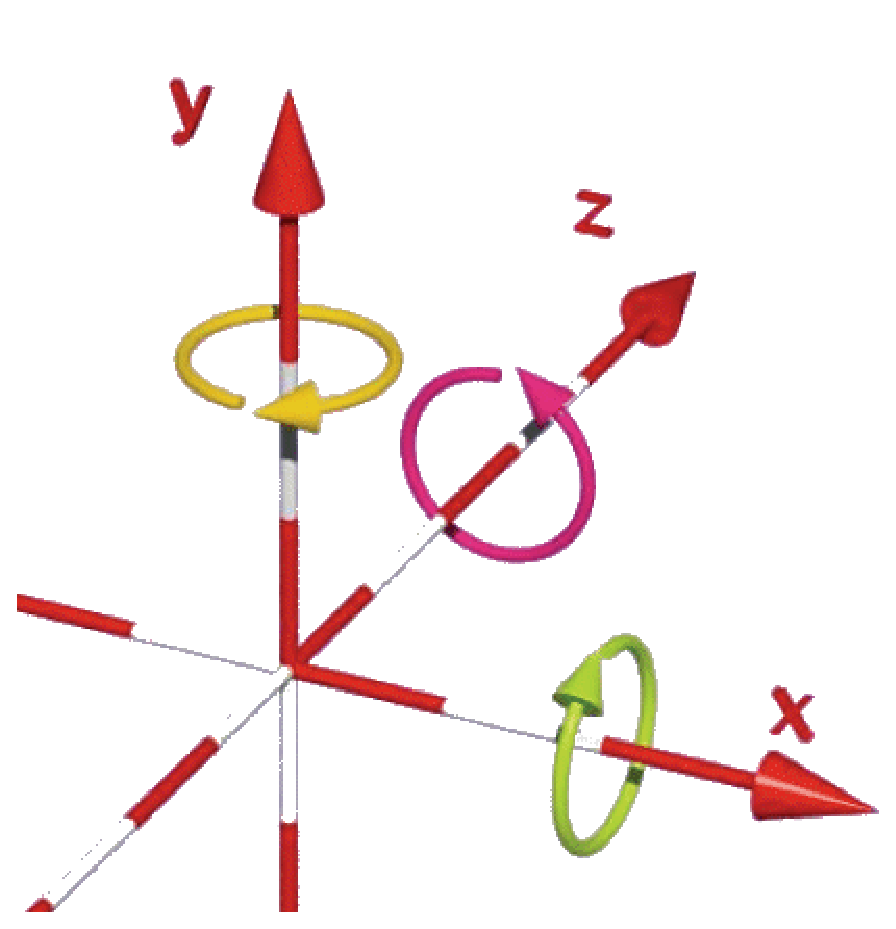
\includegraphics[width=3.2cm]{coordinate_system_white}
\caption{Left handed coordinate system.}\label{coord}
\end{center}
\end{figure}
The coordinate system is left handed, with the $y$ axis pointing
upwards, and the depth axis $z$ (cf. Figure~\ref{coord}). Input
and output files are:

\footnotetext[1]{stating
  with \texttt{XXX} = 000, 001,\dots, until no more files are
  found in the specified directory.}

\begin{enumerate}
\item The 3D scan files (\texttt{scanXXX.3d})\footnotemark[1]\
  have to be of the following structure:\\ The first line
  contains the scan's resolution (w x b), followed by lines of
  data points (x, y, z).
%
\item The pose files (\texttt{scanXXX.pose})\footnotemark[1]\ associated with each
  3D scan contain information of the estimated pose of the
  respective scan as given by, e.g., odometry. The first line
  contains the 3 translatorial positions ($x$, $y$, $z$), the
  second the rotations pitch, yaw and roll ($\theta_x$,
  $\theta_y$, $\theta_z$ around the respective axis) in deg.\\
  Values that are not estimated by the robot (odometry) can be
  set to 0 and are extrapolated as described by Eq.~\eqref{extrapol}.
%
\item The SLAM program generated files \texttt{scanXXX.frames},
  consisting of the transformations computed from the scan
  matching. Each line contains a $4 \times 4$ OpenGL-style
  matrix. The very last matrix is the final transformation for
  registering the scan into the common coordinate system.
  
  The matrix is stored in the following format:
  \begin{quote}
  $(R[1,1], R[1,2], 0, R[1,3], 0, R[2,1], R[2,2], R[2,3], 0,
  R[3,1], R[3,2], R[3,3], 0,$\\$t[1], t[2], t[3], 1),$
  \end{quote}
  with $R[x,y]$ the $(x,y)$-th entry of the rotation matrix $\M R$, and
  $t[x]$ the $x$-th translation component of $\V t$.  
\end{enumerate}

\section{Requirements}

All executables can be compiled and used both with Linux and Windows.

\begin{description}
\item[Linux:] The system was developed and tested under Linux 9.1 with
  the g++ compiler version 3.3.3. As additional library,
  \texttt{OpenGL} and \texttt{glut} have to be installed, which
  should be included in your Linux distribution (tested with
  freeglut 2.2.0-78).\\
  To compile, type in \texttt{make} in the main directory. The
  executables are generated in the \texttt{./bin} directory.
\item[Windows:]
  The system was tested with the C++ compiler from Microsoft Visual
  Studio.NET 2005.
  To compile, load the respective project file (\texttt{.sln})
  from the directory \texttt{.$\backslash$Visual\_Studio\_Projects$\backslash$}.
  The executables are generated in the respective \texttt{Debug}
  or \texttt{Release} directories, depending on your compiler settings.\\
  Precompiled versions can be found in the \texttt{./bin}
  directory, too. If moving the executables, take care about the \texttt{glut}
  directory as well.
\end{description}

\section{Usage}

For a detailed explanation about the programs' usage, just start
the respective binary.  Both applcations can be configured by a
set of command line parameters, which are explained when starting
the program as mentioned above.

Especially, take care of the reduction parameters
\texttt{-r}/\texttt{-R} of the SLAM system: Without using one of
those, the registration is being slowed down tremendously due to
taking \emph{all} data points as input. Other potentially
critical parameters are the maximal distance of points that may
form corresponding point pairs (matrix entries $w_{ij}$,
parameter \texttt{-d}), as well as the maximal range distance of
points used for scan matching or displaying (\texttt{-m}),
especially used for eliminating outliers (i.e., data points with
the maximal range distance of the range finder).

\bibliographystyle{plain}
\bibliography{diss,paper,diplom}

\end{document}